\subsection{Control deviation}\label{chapter_controlDeviationIMPL}

After calculating the state variable feedback, the dynamic behavior of the quadrocopter is fine, but the quadrocopter will not fly. There is something missing - the pre-intensivication factors. In this MIMO system, each input variable \textit{rpsi\_set}, \textit{theta\_set} and \textit{phi\_set} influences each of the three control paths. But not in the same intensity. 

First, the set variables are standardized, so that the range of the input values from -128 to 128 now reaches from -0.75 to 0.75. This is necessary, because the angels \textit{theta} and \textit{phi} are calculated in rad and the stationary throughput is calculated being one. That means, a maximum angle of approximately 45\textdegree is reached. Maybe it sounds very little, but believe - it is not. The yaw rate \textit{rpsi} is calculated in $rad/s$ so this value of 0.75 (45\textdegree/s) sounds nice for that purpose, too. 

Calculating the pre-intensification factors is not very complex. The following little code snippet shows that.

\begin{lstlisting}
KV = -(System.c * A_CL^-1 * System.b)^-1;
KV = KV';             
\end{lstlisting}

The result is the following matrix.

\begin{align}\label{eq:kv}
\bordermatrix[{[]}]{
	  				&  rpsi\_Path & theta\_Path & phi\_Path \cr
rpsi\_set 	&  7.27 & -0,32 & 0 \cr
theta\_set	&  0 & 79.36 & 0 \cr
phi\_set		& -0,57 & 0,03 & 65.05 \cr
}
\end{align}

Looking closer at the matrix reveals that these factors are nearly the same as the state variable feedback factors.

The final step is the implementation in Simulink. This part is the red one in the overview figure \ref{fig:SS_overview}. 

\begin{figure}
	\centering
		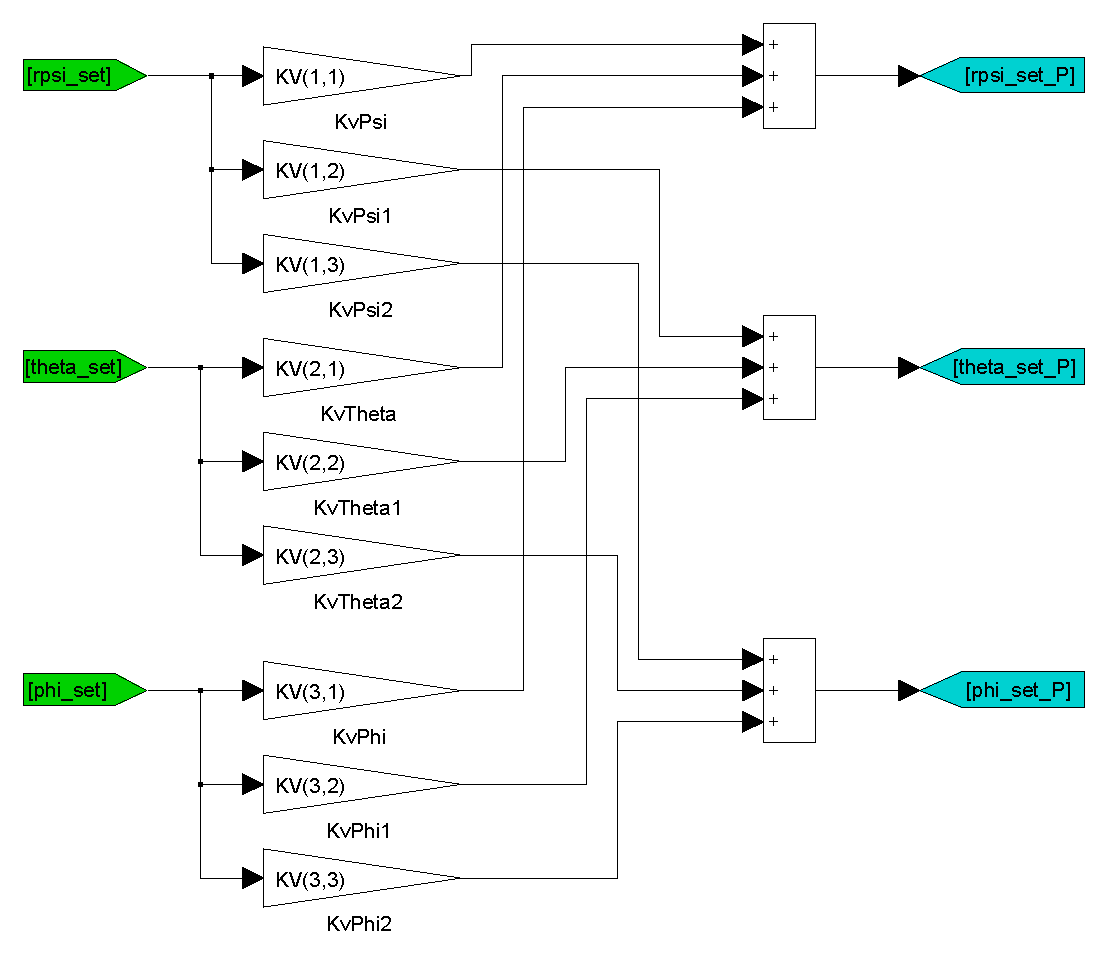
\includegraphics[width=0.80\textwidth]{03_Grafiken/SS_Pre.pdf}
	\caption{Pre-intensification factors for the different control paths}
	\label{fig:SS_Pre}
\end{figure}

Figure \ref{fig:SS_Pre} shows a detailed look at that part. The input values, marked green, are the standardized set values from the remote control. The output values, marked cyan, are the calculated set values for each path, but including the influence of the other set values.

At this step of development the continuous state space controller is finished as figure \ref{fig:Abstract} shows. The simulation results can be found in chapter (\ref{chapter_TEST}).